
\medskip

\begin{minipage}{0.42\linewidth}
Le centre Pompidou est un musée d'art contemporain à Paris. Pour accéder aux étages, il faut utiliser un ensemble d'escalators extérieurs appelé \og chenille \fg.

La chenille est composée de 5 escalators tous identiques (traits épais sur la figure ci-dessous) et de 6 passerelles horizontales toutes identiques (traits fins horizontaux sur la figure ci-dessous).
\end{minipage}\hfill
\begin{minipage}{0.56\linewidth}
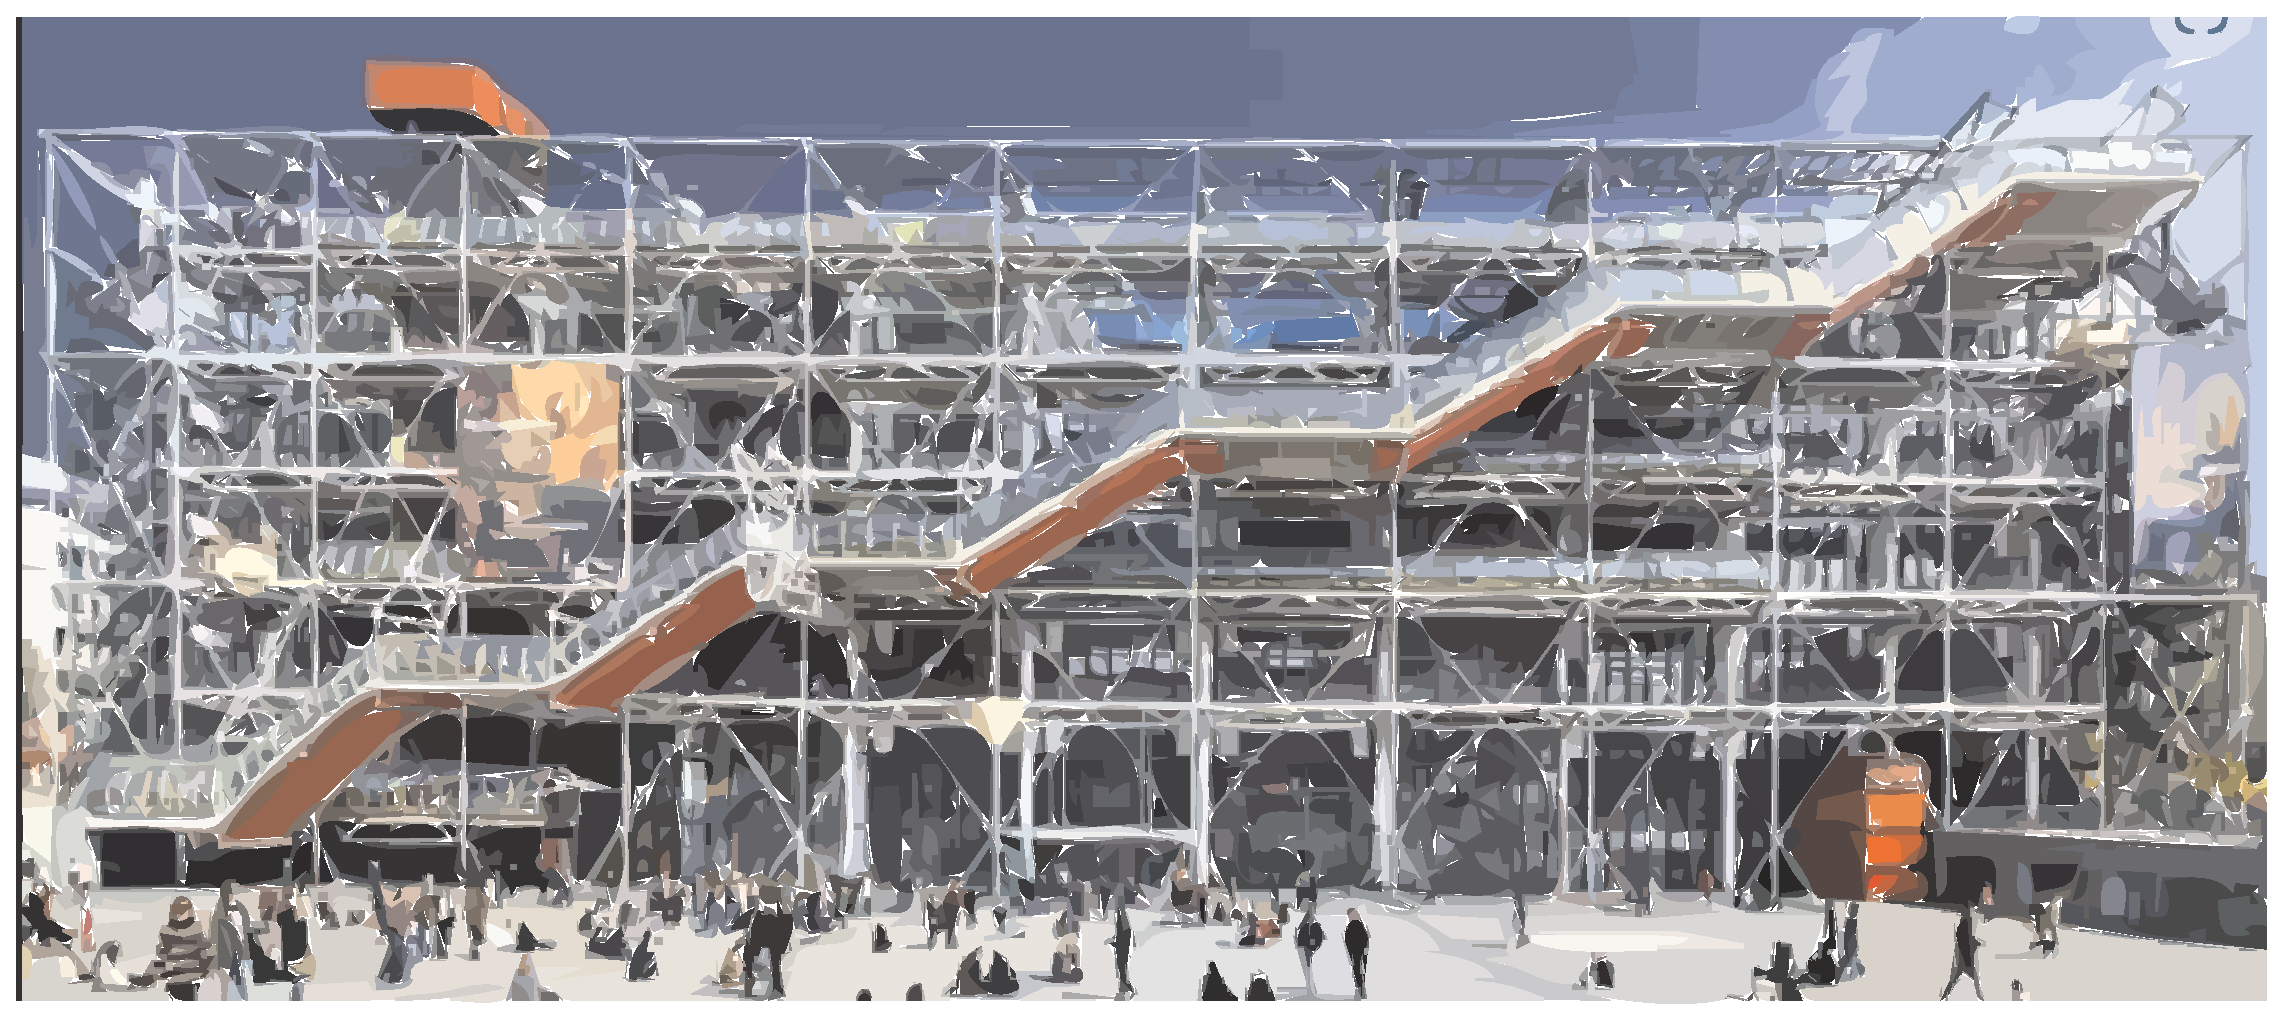
\includegraphics[width=8cm]{Pomp}
\end{minipage}

\begin{center}
\psset{unit=1cm,arrowsize=2pt 3}
\begin{pspicture}(13.5,4.6)
%\psgrid
\psline{<->}(0,0.2)(12.1,0.2)\uput[d](6.05,0.2){135 m}
\psline{<->}(12.7,0.6)(12.7,3.6)\uput[r](12.7,2.25){32 m}
\def\esca{\psline[linewidth=0.5pt](0,0)(1.1,0)\psline[linewidth=0.2pt](0.5,-0.1)(0.5,0.1)\psline[linewidth=0.2pt](0.6,-0.1)(0.6,0.1)\psline[linewidth=1.25pt](1.1,0)(2.2,0.6)\psline[linewidth=1.25pt](1.65,0.35)(1.75,0.25)}
\multido{\n=0.0+2.2,\na=0.6+0.6}{5}{\rput(\n,\na){\esca}}
\psline[linewidth=0.2pt](11,3.6)(12.1,3.6)
\psline{<->}(11,4)(12.1,4)\uput[u](11.55,4){12,5 m}
\psline[linewidth=1.5pt,linestyle=dotted](5.5,1.8)(6.6,1.8)(6.6,2.4)\uput[d](6.05,1.8){$p$}
\uput[r](6.6,2.1){$h$}
\psline[linewidth=0.2pt](11.5,3.7)(11.5,3.5)\psline[linewidth=0.2pt](11.6,3.7)(11.6,3.5)
\psline[linewidth=1.5pt,linestyle=dotted](1.1,0.6)(12.7,0.6)
\end{pspicture}
\end{center}

\medskip

\begin{enumerate}
\item À l'aide de la figure ci-dessus :
	\begin{enumerate}
		\item Vérifier que la profondeur $p$ de chaque escalator est égale à $12$ m
		\item Calculer la hauteur $h$ de chaque escalator
	\end{enumerate}	
\end{enumerate}
\begin{minipage}{0.62\linewidth}
\begin{enumerate}[resume]
\item À l'aide du triangle RST ci-contre :
	\begin{enumerate}
		\item Prouver que la longueur ST d'un escalator est de $13,6$ m.
		\item Montrer que la mesure de l'angle formé par l'escalator avec l'horizontale (c'est-à-dire l'angle $\widehat{\text{RST}}$ arrondie au degré est de $28\degres$.
	\end{enumerate}
\end{enumerate}
\end{minipage}\hfill
\begin{minipage}{0.36\linewidth}
\psset{unit=1cm}
\begin{pspicture}(4.8,2.4)
\psline[linewidth=1.5pt,linestyle=dotted](0.2,0.2)(3.8,0.2)(3.8,1.8)%SRT
\psline[linewidth=1.5pt](0.2,0.2)(3.8,1.8)
\uput[dr](3.8,0.2){R} \uput[dl](0.2,0.2){S} \uput[ur](3.8,1.8){T} \uput[d](2,0.2){12 m} \uput[r](3.8,1){6,4 m}
\end{pspicture}
\end{minipage}

\begin{enumerate}[resume*,start=3]		
\item Sabine veut représenter la chenille grâce au logiciel Scratch.

Elle a écrit le programme qui est donné sur le document joint. On précise que : 1 pas du logiciel correspond à 1 m dans la réalité.

Compléter les lignes 6, 7, 9, et 10 sur le document (à rendre avec la copie), afin d'obtenir le tracé ci-dessous de la chenille :

\begin{center}
\psset{unit=0.8cm,arrowsize=2pt 3}
\begin{pspicture}(13.5,4.6)
\def\esca2{\psline[linewidth=0.5pt](0,0)(1.1,0)\psline[linewidth=1.25pt](1.1,0)(2.2,0.6)}
\multido{\n=0.0+2.2,\na=0.6+0.6}{5}{\rput(\n,\na){\esca2}}
\psline[linewidth=0.2pt](11,3.6)(12.1,3.6)
\end{pspicture}
\end{center}

Rappel : \og S'orienter à 90 \fg{} signifie que l'on est orienté vers la droite
\end{enumerate}


\begin{center}

\textbf{\large À compléter et à rendre avec la copie}

\end{center}

\bigskip

\textbf{Ex 5 question 3 :}

\bigskip

\begin{center}
\begin{scratch}[scale=1.75, num blocks]
\blockinit{quand \greenflag est cliqué}
\blockpen{effacer tout}
\blockmove{s'orienter à \ovalnum{90}}
\blockmove{aller à x: \ovalnum{-120} y: \ovalnum{-60}}
\blockpen{stylo en position d'écriture}
\blockrepeat{répéter \ovalnum{} fois}
{
\blockmove{avancer de \ovalnum{}}
\blockmove{tourner \turnleft{} de \ovalnum{28} degrés}
\blockmove{avancer de \ovalnum{}}
\blockmove{tourner \turnright{} de \ovalnum{} degrés}
}
\blockmove{avancer de \ovalnum{12,5}}
\blockpen{relever le stylo}
\end{scratch}
\end{center}



